\subsection{Metodologia}
O processo é conduzido da seguinte forma: o professor acessa a extensão ESPEON em seu navegador e cadastra uma nova aula no banco de dados da aplicação. Ao final do cadastro, a extensão gera automaticamente uma expressão regular (\textit{regex}) correspondente ao título da aula, conferindo padronização à identificação da aba da conferência. Essa expressão serve como referência para o campo \textit{onlineClass}, que é utilizado pela extensão para detectar mudanças de aba durante a aula. O formulário de cadastro de aula pode ser observado na Figura~\ref{fig:figura1}, e a geração da expressão regular correspondente está ilustrada na Figura~\ref{fig:figura2}.

% \FloatBarrier
\begin{figure}[H]
\centering
\begin{minipage}{0.48\textwidth}
    \centering
    \includegraphics[width=.9\textwidth]{assets/images/formulário de aula.png}
\caption{Formulário de Cadastro de Aula}
\label{fig:figura1}
\end{minipage}\hfill
\begin{minipage}{0.48\textwidth}
    \centering
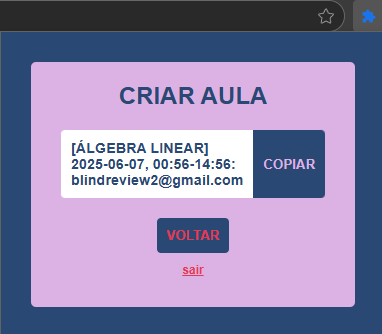
\includegraphics[width=.9\textwidth]{assets/images/aula criada.png}
\caption{Geração do Título de Aula (\textit{Regex})}
\label{fig:figura2}
\end{minipage}
\end{figure}

Em seguida, o professor cria uma reunião no Microsoft Teams utilizando o título gerado, obtendo o \textit{link} correspondente, que deve então ser disponibilizado à turma. Os alunos autenticam-se na extensão com seus \textit{e-mails} institucionais e submetem o \textit{link} da aula por meio da interface da aplicação. O rastreamento das atividades inicia-se, podendo ser finalizado no botão de \textit{stop}. A etapa de inscrição em aula está ilustrada na figura ~\ref{fig:figura3}.

% \FloatBarrier
\begin{figure}[ht]
\centering
\includegraphics[width=.5\textwidth]{assets/images/submissão.png}
\caption{Submissão da Aula à Extensão pelos Alunos}
\label{fig:figura3}
\end{figure}

Ao término da aula, o aluno finaliza o monitoramento, e as chamadas ao banco são encerradas. Esse monitoramento gera \textit{logs} de atividade que vão compor os relatórios de aula.
Esse documento contém métricas relacionadas à atenção e engajamento dos alunos, conforme ilustrado na Tabela~\ref{tab:table1}, e será de grande valia para futuros estudos de laboratório.

% \FloatBarrier
\begin{table}[H]
\centering
\caption{Métricas utilizadas para avaliação de atenção e engajamento}
\label{tab:table1}
\begin{tabular}{|l|p{10cm}|}
\hline
\textbf{MÉTRICA} & \textbf{DESCRIÇÃO} \\
\hline
Tempo de Inatividade & Tempo total gasto fora da guia onde ocorre a aula. \\
\hline
Tab Swap & Tempo gasto trocando de abas durante a aula. \\
\hline
Área do Conhecimento & Segmentação dos dados por área do 
conhecimento da disciplina ministrada. \\
\hline
Tempo de Foco & Tempo máximo de foco contínuo na guia onde ocorre a aula. \\
\hline
Aba Silenciada & Tempo máximo em que a aba da aula permaneceu silenciada. \\
\hline
Permissionamento & Verificação de permissionamento para uso de periféricos de áudio e vídeo. \\
\hline
Streaming de Periféricos & Verificação de uso ativo (streaming) dos periféricos de áudio e vídeo. \\
\hline
\end{tabular}
\end{table}


